\section{Arbeitsgrundlagen}

(Auszug aus der Aufgabenstellung\cite{ref:aufgabenstellung})

Die Ausbreitung von Licht und deren Wechselwirkung mit  materiellen  K\"orpern
kann in zwei Bereichen aufgeteilt werden.


\subsection{Wellentheorie der Elektromagnetischen Strahlung}

Licht wird als elektromagnetische  Welle  modelliert,  darstellbar  durch eine
kontinuierliche Wellenfunktion,  zum  Beispiel  $\vec{E}(\vec{r},t)$ f\"ur die
elektrische Feldst\"arke.

Zu  dieser  Aufgabe  relevante  charakteristische  Gr\"ossen  sind  dabei  die
Wellenl\"ange  $\lambda$  und  die  Frequenz  $f$, wobei sich  die  Welle  mit
Lichtgeschwindigkeit $c$ ausbreitet.

\begin{equation}
    \lambda \cdot f = c
\end{equation}


\subsection{Quantentheorie der elektromagnetischen Strahlung}

Licht  wird  als  ein  Strom  von  Photonen $\gamma$ interpretiert, welche  in
\textbf{individuellen Quantenprozessen} mit  einzelnen  Atomen, Elektronen und
so weiter  in  wechselwirkung treten. Diese unterliegt dem Zufall, weshalb nur
\textbf{Wahrscheinlichkeitsaussagen} gemacht werden k\"onnen.

Zu dieser Aufgabe relevante charakteristische Gr\"ossen sind dabei die Energie
$E_{\gamma}$ und die Plank'sche Konstante  $h$  (welches wir in diesem Versuch
bestimmen werden).

\begin{equation}
    E_{\gamma} = h \cdot f = \frac{h \cdot c}{\lambda}
\end{equation}


\subsection{Der Photoeffekt}

Beim Photoeffekt  handelt  es  sich  um  die Absorption von Lichtquanten durch
Atome, Mole\"ule, Festk\"orper, bei der  das  Photon verschwindet und ein Teil
seiner  Energie  auf  ein  Elektron  \"ubertragen  wird.  Im Falle von Atomen,
Mole\"ulen  enstehen  im  ersten Momen freie Elektronen mit kinetische Energie
$E_k = E_{\gamma} -  E_B$  (Die  am  Prozess  beteiligten  Atome  sind so viel
schwerer, dass ihre Energie vernachl\"assigt werden kann), welche sich dann an
andere  Teilchen  anlagern   k\"onnen.   $E_B$  ist  die  Bindungsenergie  des
Elektrons.  Im Falle der Wechselwirkung mit Festk\"orpern wird  unterschieden:


\subsubsection{\"Ausserer Photoeffekt}

Die Lichtquanten ``schlagen'' aus der Oberfl\"ache von  Metallen, Metalloxiden
und  Halbleitern  Photoelektronen  heraus. Zur Befreiung eines Elektrons  muss
dessen  Bindungsenergie  aufgewendet  werden,  man  bezeichnet  sie  hier  als
Austrittsarbeit  $W_a$.  Es ist klar, dass  die  Photonenenergie  $E_{\gamma}$
mindestens  gleich  $W_a$  sein muss, damit der Effekt eintritt.  Der  Prozess
spielt   sich   in   einer   d\"unnen  Oberfl\"achenschicht  ab,  welche   der
Eindringtiefe der Photonen entspricht1) . Deshalb erleiden die Photoelektronen
vor dem Austritt durch Wechselwirkung  mit dem Kristallgitter unterschiedliche
Energieverluste und verlassen die Oberfl\"ache mit variabler  kinet.  Energie.
Der Maximalwert ist gegeben durch die Gleichung:

\begin{equation}
    E_k = E_{\gamma} - W_a = h \cdot f - W_a
\end{equation}

welche erstmals von  \textit{Einstein}  formuliert  wurde. Die Austrittsarbeit
ist   eine   Oberfl\"acheneigenschaft   und   nur   bei   gr\"osster  Reinheit
materialspezifisch.   Adsorbierte  Gase,  Oxidfilme  und  andere   Fremdstoffe
k\"onnen den  Wert erheblich ver\"andern. Schichten, welche zur Umwandlung von
Strahlung  in   einen   Photoelektronenstrom   dienen,   bezeichnet   man  als
Photokathoden; wird eine solche  mit  einem  Sekund\"arelektronenvervielfacher
(engl. \textit{Multiplier}) kombiniert,  erh\"alt  man  einen Photomultiplier,
den empfindlichsten Strahlungsdetektor.


\subsubsection{Innerer Photoeffekt}

Die in einen  Halbleiter  eindringenden Lichtquanten produzieren zus\"atzliche
Ladungstr\"ager, wir unterscheiden:

Photoleiter     (Photowiderst\"ande):     bei    Bestrahlung     nimmt     die
Ladungstr\"agerdichte und damit die Leitf\"ahigkeit zu. Beispiele sind: CdS im
Sichtbaren, InAs und InSb im nahen IR, dotiertes Ge bis ins  ferne  IR.  Wegen
ihrer  Einfachheit  werden  solche  Elemente  f\"ur  zahlreiche   Messaufgaben
eingesetzt.   Photodioden:  im  Bereich  des  p-n-\"Uberganges  erzeugen   die
absorbierten Photonen Elektron-Loch- Paare, welche im  elektrischen  Feld  der
Raumladungszone  getrennt  werden. Ohne  \"aussere  Quelle  wird  die  p-Seite
positiv und  die  n-Seite  negativ aufgeladen, es entsteht eine Photospannung,
die  maximal entgegengesetzt gleich der Diffusionsspannung $U_d$ werden  kann.
Bei Belastung  fliesst ein entsprechender Strom ( Elementbetrieb) zum Beispiel
bei Solarzellen. Wird eine \"aussere Spannung  in  Sperrrichtung  angelegt, so
fliesst  in  dieser  Richtung  ein Photostrom,  der  streng  proportional  zur
auftreffenden  Strahlungsleistung   ist  (  Diodenbetrieb),  angewendet  f\"ur
Photodetektoren.  Diese   Vorg\"ange  laufen  nat\"urlich  nur  ab,  wenn  die
Photonenenergie  einen  materialspezifischen  Schwellenwert   \"uberschreitet,
welcher  der  Freisetzung  eines  ans   Kristallgitter   gebundenen  Elektrons
entspricht.  In  eigenleitendem Material ist der energetische Abstand zwischen
Leitungs-  und  Valenzband = Breite der Bandl\"ucke (engl. \textit{gap}) $E_g$
massgebend.  Dies  ergibt  die  langwellige Grenze  der  Photoempfindlichkeit.


\subsection{Leuchtdioden, physikalische Grundlagen}

Die Lichtemission von  Atomen,  Molek\"ulen  und  Festk\"orpern  kommt dadurch
zustande, dass Elektro- nen von h\"oheren in tiefer liegende Energiezust\"ande
\"ubergehen.  Bei  jedem  einzelnen  Quantenprozess wird die  Energiedifferenz
$\Delta  E$  als   einzelnes   Photon   mit   der   Wellenl\"ange  $\lambda  =
\frac{hc}{\Delta  E}$  ausgesandt.  Leuchtdioden   (Lumineszenzdioden,   engl.
\textit{light  emitting diodes}, abgek\"urzt LED) sind spezielle, hochdotierte
p-n-Dioden,  vorwiegend  III/V-Halbleiter wie  GaAs,  GaP  und  Mischkristalle
GaAsxP1-x,  eine  \"Ubersichtstabelle  findet sich in PI, S. 690. Fliesst  ein
Strom in  Leitrichtung,  gehen  im Bereich des p-n-\"Uberganges Elektronen vom
Leitungsband  ins Valenzband \"uber,  wobei  der  Energieunterschied  von  der
ungef\"ahren  Gr\"osse  des Bandabstandes = Bandl\"ucke  (engl.  gap)  Eg  als
Photon emittiert wird.  Wir  geben  nachfolgend  eine  kurze  Darstellung  der
Vorg\"ange am p-n-\"Ubergang, f\"ur  eine  genauere  Betrachtung  sei  auf die
Literatur, z.B. PI, 9.2.3.2 und 9.2.3.3, S. 665 ff. verwiesen.

\subsubsection{Vorg\"ange am p-n-\"Ubergang}

Bringen  wir  ein  p-   und  ein  n-leitendes  Halbleitermaterial  in  Kontakt
\ref{fig:pn},   so   bestehen   an   der   Grenzfl\"ache   f\"ur   die  beiden
Ladungstr\"agersorten,    Elektronen     und    L\"ocher,    vorerst    grosse
Konzentrationsgef\"alle   .    Diese    bewirken,    dass    die    jeweiligen
Majorit\"ats-Ladungstr\"ager \"uber die Grenze ins Nachbargebiet diffundieren:
die  Elektronen  ins  p-Gebiet,  die  L\"ocher  ins  n-Gebiet. Dort  ist  ihre
Lebensdauer kurz, denn sie rekombinieren mit den  dort  zahlreich  vorhandenen
Majorit\"ats- Ladungstr\"agern der jeweils  anderen Sorte. Wegen der Verarmung
an   Majorit\"ats-Ladungstr\"agern   bildet   sich   auf   der   n-Seite   des

\"Ubergangs eine positive, auf der p-Seite eine negative, ortsfeste Raumladung
$\rho(x)$  aus,  welche  je  aus den nicht mehr kompensierten  Akzeptor-  bzw.
Donator-Ionen besteht. Das damit verbundene elektrische Feld  $E(x)$ hat einen
Driftstrom zur Folge, der entgegen dem Diffusionsstrom  fliesst,  und  solange
anw\"achst,   bis   der  stromlose  Gleichgewichtszustand  erreicht  ist.  Die
zugeh\"orige Potentialdifferenz  heisst  Diffusionsspannung  $U_d$ und ist ein
wichtiger Parameter des p-n-\"Ubergangs.

\begin{figure}[H]
    \centering
    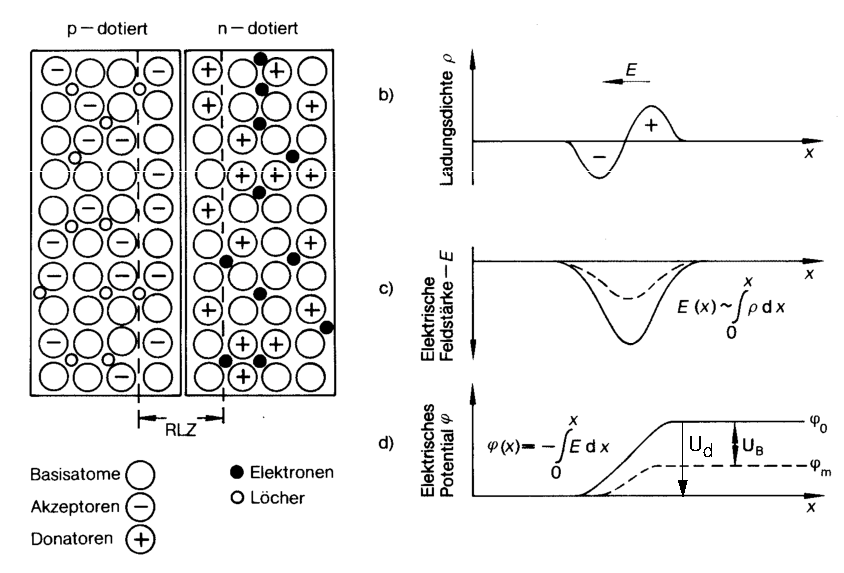
\includegraphics[width=.8\linewidth]{images/pn}
    \caption{(Aus HP 8.4)}
    \label{fig:pn}
\end{figure}

Legt man eine  \"aussere  Spannung  in  Leitrichtung $p \to n$ an, so wird die
Potentialbarriere reduziert auf den Wert $U_d - U$ , die Raumladungszone (RLZ)
wird schmaler und der Driftstrom kleiner.  Es  fliesst also ein Nettostrom von
Ladungstr\"agern   \"uber   den  p-n-\"Ubergang  und  rekombiniert  wie   oben
beschrieben -- im p-Gebiet  die  eingedrungenen  Elektronen  mit L\"ochern, im
n-Gebiet die  eingedrungenen L\"ocher mit Elektronen. Dieser Durchlassstrom in
Leitrichtung wird im p-Gebiet von  L\"ochern,  im  n-Gebiet von Elektronen, im
p-n-\"Ubergang von beiden  Ladungstr\"agersorten  getragen. Solange $U < U_d$,
bestimmt  die  Potentialdifferenz  in  der RLZ den Strom, der in  diesem  Fall
exponentiell verl\"auft.  Wenn $U > U_d$ wird der p-n-\"Ubergang ``flach'' und
der  Materialwiderstand  beidseits des \"Ubergangs wird bestimmend, die  Diode
verh\"alt sich dann  wie  ein  Ohm'scher  Widerstand.  Der steile Stromanstieg
setzt  bei  $U  \approx  U_d$  ein,   dort   beobachtet   man  den  Knick  der
Diodenkennlinie. Polt man die  \"aussere  Spannung in Sperrrichtung $n \to p$,
so erh\"oht man  die  Potentialbarriere  und  verbreitert  die Raumladungszone
(RLZ). Es  fliesst  ein winziger Sperrstrom, der dadurch bedingt ist, dass ein
kleiner  Bruchteil  der Ladungstr\"ager gen\"ugend thermische Energie hat,  um
die  Barriere  zu  \"uberqueren,  er   nimmt  mit  der  Temperatur  stark  zu.


\subsubsection{Leuchtdioden}

Rekombination   der   Ladungstr\"ager  heisst  im  Klartext:  \"Ubergang   von
Elektronen  aus  dem  Leitungsband  ins  Valenzband.  Die  dabei frei werdende
Energie  wird  bei  der  normalen  Diode  in   W\"arme  umgewandelt,  bei  der
Leuchtdiode hingegen wird sie \"uberwiegend als Licht  frei. Die nebenstehende
Figur veranschaulicht  die Vorg\"ange am p-n-\"Ubergang. Der aufmerksame Leser
merkt: Dieser Vorgang ist der Umkehrprozess zum inneren Photoeffekt, wo in der
(an   Ladungstr\"agern  verarmten)  Raumladungszone  einer  in   Sperrrichtung
gepolten Diode Elektron-Lochpaare erzeugt werden.

\clearpage
\begin{wrapfigure}{r}{.5\linewidth}
    \centering
    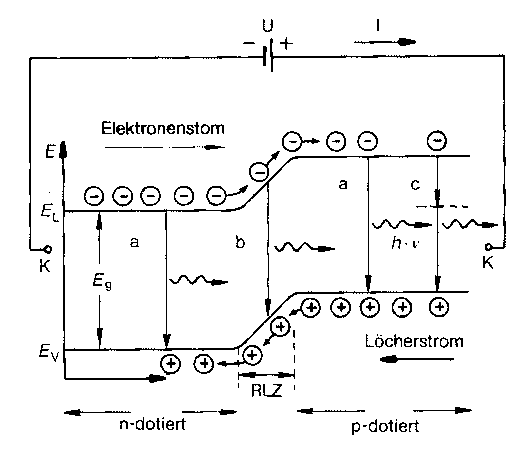
\includegraphics[width=\linewidth]{images/led}
    \caption{(aus HP 8.6)}
    \label{fig:led}
\end{wrapfigure}

Die Rekombinationsrate ist  proportional zum Strom, n\"aherungsweise gilt dies
auch f\"ur die  Pro  duktionsrate  der  Photonen.  Allerdings  tritt  nur  ein
Bruchteil davon aus, wof\"ur u.a. der grosse Brech ungsindex des Materials ($n
\approx  3.5$)  verantwortlich  ist,   schon   bei   einem   relativ   kleinen
Einfallswinkel auf die Grenzfl\"ache  tritt  Totalreflexion  auf. Das Spektrum
des  emittierten   Lichtes   wird   von   der   inneren   Energiestruktur  des
Halbleiter-Materials    bestimmt,    d.h.   vom   Abstand   zwischen   Valenz-
undLeitungsband-Kanten  $E_g$,  von  der  energetischen  Lage  der Akzeptoren,
Donatoren   und  anderer  St\"orstellen.  Eine   grosse   Zahl   verschiedener
Rekombinationsprozesse  tr\"agt  zur   Lichtemission   bei:  Leitungsband  -->
Valenzband, Donator --> Valenzband,  Leitungsband  -->  Akzeptor,  Donator -->
Akzeptor  usw..  Bei  h\"oheren Temperaturen verschwinden die Einzelheiten und
das Spektrum  nimmt eine mehr oder weniger glockenf\"ormige Form an. F\"ur die
h\"aufigste Quantenenergie kann man n\"aherungsweise den Wert $E_{\gamma} =  h
c  \lambda  \approx  E_g$  erwarten.  Es  stellt  sich   die   Frage,  welcher
Zusammenhang zur Kennlinie  der  Leuchtdiode  besteht.  Die Diffusionsspannung
$U_d$ h\"angt in komplizierter Weise vom Material,  seiner Dotierung sowie dem
geometrischen Aufbau der Diode ab. Weil Leuchtdioden hoch dotiert sind, liegen
die Fermi-Energien nahe den Bandkanten und $e \cdot U_d$ ist ungef\"ahr gleich
dem Bandabstand $E_g$, in der Regel etwas  kleiner.  Wir  haben  oben gesehen,
dass $U_d$ etwa der Knickspannung UK  der  Kennlinie  entspricht. Die messbare
Knickspannung  und die Wellenl\"ange des Emissionsmaximums einer  LED  sollten
also n\"aherungsweise der Beziehung:

\begin{equation}
    e \cdot U_K \approx E_{\gamma} = h c \lambda
\end{equation}

gen\"ugen, meistens findet man einen um etwa \SI{10}{\percent} kleineren Wert.

